\section{Sisteme de recomandare}

\subsection{Noțiuni generale}

Sistemele de recomandare au scopul de oferi sugestii cât mai relevante de articole utilizatorilor unei platforme pe baza unor strategii. Un sistem de recomandare poate folosi una sau mai multe strategii de recomandare după cum vom vedea în continuare. În cazul în care se folosesc cel puțin două strategii, sistemul de recomandare devine un sistem de recomandare hibrid. Prin folosirea mai multor strategii se urmărește ca fiecare strategie să vină în completarea celorlalte strategi cu avantajele sale. De cele mai multe ori, în implementarea unui sistem de recomandare, se folosește tehnica de filtrare coloborativă împreună cu o altă strategie de recomandare \hyperlink{ErionCanoMaurizioMorisio}{[4]}.

\subsection{Strategii de recomandare}

\subsubsection*{Filtrarea coloborativă}

Filtrarea coloborativă se bazează pe faptul că utilizatorii care au în prezent preferințe similare vor avea și în viitor preferințe destul de similare. Această abordare folosește ratingurile pe care le dau utilizatorii sau oricare altă formă de a da un feedback, îmi place/nu îmi place, pentru a identifica preferințele comune dintre grupurile de utilizatori. Odată identificate preferințele se generează recomandări pe baza similarităților dintre utilizatori. 

Dezavantajul acestei strategii apare în momentul în care în sistem intră un nou utilizator. Datorită faptului că utilizatorul este nou, sistemul nu are un istoric al preferințelor lui, iar în consecință nu îl poate asigna unui grup de utilizatori pe baza preferințelor \hyperlink{ErionCanoMaurizioMorisio}{[4]}.
\begin{figure}[!h]
	\centering
	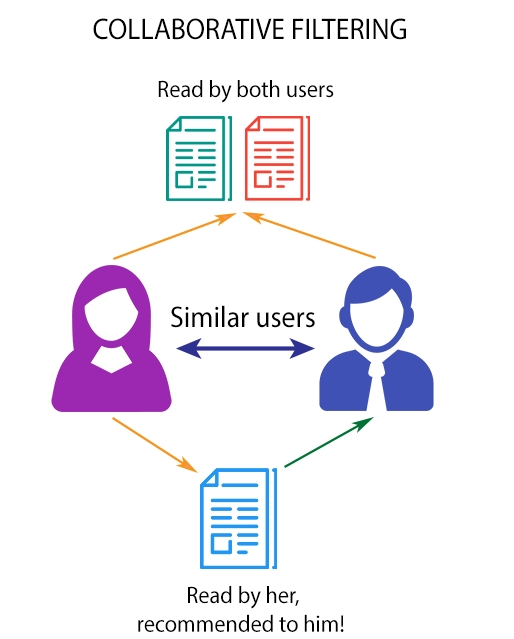
\includegraphics[max width=10cm,max height=10cm,keepaspectratio]{img_2_1}
	\caption[Filtrarea coloborativă]{Filtrarea coloborativă. Imagine preluată din \hyperlink{datameetsmedia}{[5]}.}
\end{figure} 

\subsubsection*{Filtrarea bazată pe conținut}

Filtrarea bazată pe conținut pleacă de la premisa că utiliztorii cărora le-au plăcut articole definite de anumite caracteristici în trecut, vor aprecia aceleași tip de articole și în viitor. Această abordare folosește caracteristicile articolelor pentru a le compara cu profilul utilizatorilor și a oferi recomandări. Calitatea recomandărilor rezultate folosind această strategie este influențată de setul de caracteristici ales pentru articole. Similar cu filtrarea coloborativă, filtrarea bazată pe conținut prezintă dezavantaje în momentul în care în sistem intră un nou utilizator fără istoric \hyperlink{ErionCanoMaurizioMorisio}{[4]}.
\begin{figure}[!h]
	\centering
	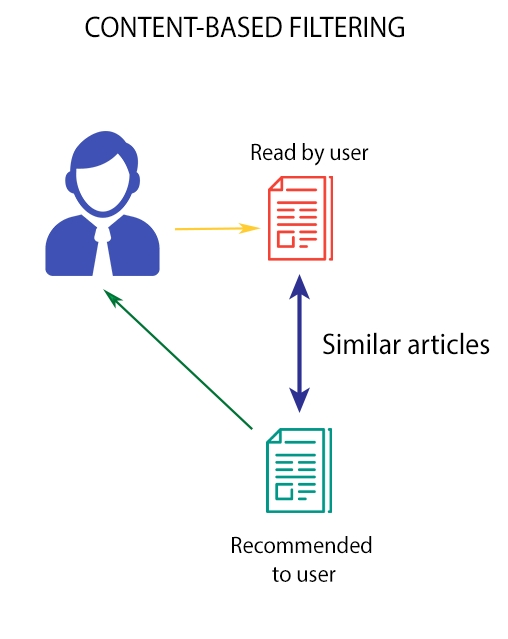
\includegraphics[max width=10cm,max height=10cm,keepaspectratio]{img_2_2}
	\caption[Filtrarea bazată pe conținut]{Filtrarea bazată pe conținut. Imagine preluată din \hyperlink{datameetsmedia}{[5]}.}
\end{figure} 

\subsubsection*{Filtrarea demografică}

Filtrarea demografică folosește atribute precum vârsta, genul, educația, etc. pentru a identifica categoriile de utilizatori. Nu prezintă dezavantaje atunci când apar noi utilizatori în sistem și nu se folosește de ratinguri, sau alt sistem de feedback, pentru a face recomandări.

Dezavantajul este reprezentat de faptul că procesul de colectare al datelor demografice poate fi îngreunat de legislație, fapt ce reprezintă o limitare a acestei metode \hyperlink{ErionCanoMaurizioMorisio}{[4]}.

\subsubsection*{Filtrarea bazată pe cunoștințe}

Filtrarea bazată pe cunoștințe folosește cunoștințele despre utilizatori și articole pentru a spune ce articole îndeplinesc cerințele utilizatorilor și genereaza recomandări în consecință. Filtrare bazată pe cunoștințe are la bază constrângeri și este capabilă să recomande chiar și articole complexe care nu sunt cumpărate atât de des, precum mașini sau case \hyperlink{ErionCanoMaurizioMorisio}{[4]}.

\subsection{Funcții de eroare}

\subsubsection*{BPR: Bayesian Personalised Ranking}

Este o metodă ce se bazează pe feedback implicit (click-uri, ratinguri, achiziții, vizualizări). Exită multe metode ce se bazează pe acest feedback implicit, precum matrix factorization (MF), k-nearest neighbors (kNN), însă acestea nu sunt optimizate pentru ranguri. Metoda de învățare este bazată pe gradientul descendent și este recomandată atunci când se dorește optimizarea acurateții.

Definim în continuare $U$ ca fiind mulțimea de utilizatori și $I$ ca fiind mulțimea de articole. Feedback-ul implicit este reprezentat de mulțimea $S \subseteq U \times I$. De asemenea, definim $I_u^+ := {i \in I:(u, i) \in S}$ și $U_i^+ := {u \in U:(u, i) \in S}$.
\begin{figure}[!h]
	\centering
	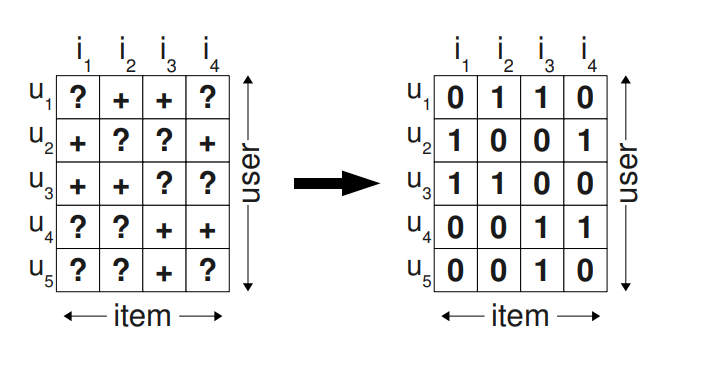
\includegraphics[max width=10cm,max height=10cm,keepaspectratio]{img_2_8}
	\caption[Matricea de interacțiuni]{Matricea de interacțiuni, mulțimea $S$. Imagine preluată din \hyperlink{SteffenRendleChristophFreudenthalerZenoGantnerLarsSchmidtThieme}{[9]}.}
\end{figure} 

O abordarea uzuală pentru recomandarea de articole este să fie estimat scorul $\hat{x}_{ui}$ care să reflecte preferința utilizatorului $u$ pentru articolul $i$. Apoi fiecare articol primește un rang după sortarea scorurilor.

Setul de antrenare (vezi figura 2.4) este definit de mulțimea $D_S := \{(u,i,j)|i \in I_u^+ \wedge j \in I \setminus I_u^+\}$ unde $(u,i,j)$ înseamnă că utilizatorul $u$ preferă articolul $i$ în detrimentul articolului $j$.
\begin{figure}[!h]
	\centering
	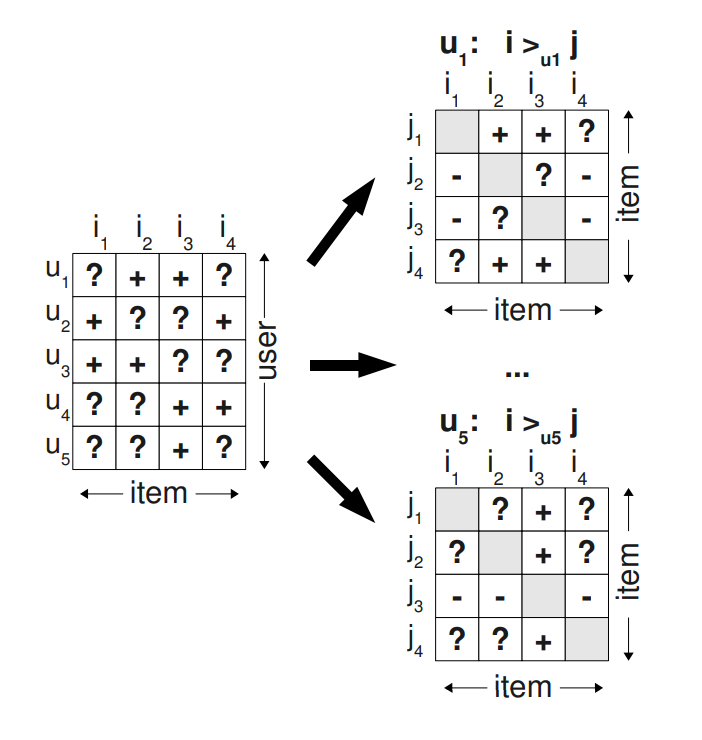
\includegraphics[max width=10cm,max height=10cm,keepaspectratio]{img_2_9}
	\caption[Setul de antrenare]{Setul de antrenare. $+$ reprezintă articolele $i$ pe care utilizatorul le preferă în locul articolelor $j$, $-$ utilizatorul preferă articolele $j$ în loc de $i$, iar $?$ reprezintă lipsa informației despre acea interacțiune. Imagine preluată din \hyperlink{SteffenRendleChristophFreudenthalerZenoGantnerLarsSchmidtThieme}{[9]}.}
\end{figure} 

Criteriul de optimizare pentru pentru rangurile personalizate este definit după cum urmează:
\begin{align}
	BPR-OPT := \sum_{(u,i,j) \in D_S} \ln{\sigma(\hat{x}_{uij})} - \lambda_\Theta||\Theta||^2
\end{align}
unde $\sigma$ este funcția sigmoid, $\sigma(x) := \frac{1}{1+e^{-x}}$, $\Theta$ reprezintă vectorul parametru al modelului care definește interacțiunea dintre utilizatorul $u$, articolul $i$ și articolul $j$, iar $\lambda_\Theta$ reprezintă parametrii de regularizare.

Cu aceste definiți putem defini și procedura de învățare a $BPR$ după cum urmează în figura 2.5:
\begin{figure}[!h]
	\centering
	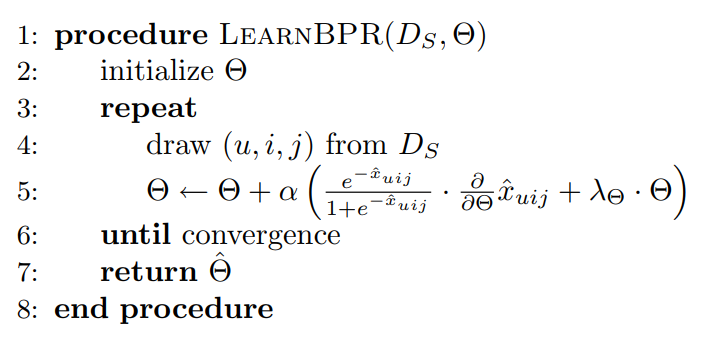
\includegraphics[max width=10cm,max height=10cm,keepaspectratio]{img_2_10}
	\caption[Procedura de învățarea BPR]{Optimizarea modelului bazată metoda gradientului descendent cu parametrul de învățare $\alpha$ și regularizarea $\lambda_\Theta$. Imagine preluată din \hyperlink{SteffenRendleChristophFreudenthalerZenoGantnerLarsSchmidtThieme}{[9]}.}
\end{figure}

\vspace{5mm}
\subsubsection*{WARP: Weighted Approximate-Rank}

Această metodă își are originile în procesarea imaginilor și anume pentru un set de reprezentări ale unor imagini $x \in R^d$ și pentru un set de reprezentări ale unor adnotări $i \in \Upsilon = \{1, ..., Y\}$ - inidici intr-un dicționar cu posibile adnotări, metoda învață să mapeze imagini din spațiul reprezentărilor într-un spațiu comun $R^D$
\begin{align}
	\Phi_{I}(x):R^d \rightarrow R^D
\end{align}
în același timp învățând și mapări pentru adnotări în același spațiu
\begin{align}
	\Phi_{W}(i):{1,...,Y} \rightarrow R^D
\end{align}

Scopul principal fiind acela de a oferi ranguri posibilelor adnotări pentru o imagine dată astfel încât cel mai mare rang să descrie cel mai bine conținutul semnatic al imaginii. 

Modelul folosit este definit în continuare:
\begin{align}
	f_{i}(x) = \Phi_{W}(i)^T \Phi_{I}(x)
\end{align}

Metoda învață să producă ranguri optimizate pentru primele adnotări din listă, ceea ce înseamnă că optimizează precizia@k.

În ceea ce privește funcția de eroare definim: $f(x) \in R^Y$ ce produce un scor pentru fiecare etichetă și unde $f_i(x)$ este valoarea etichetei $i$. Definim funcția de eroare pentru ranguri ca fiind:
\begin{align}
	err(f(x),y) = L(rank_y(f(x)))
\end{align}
unde $rank_y(f(x))$ este rangul etichetei corecte data de $f(x)$:
\begin{align}
	rank_y(f(x)) = \sum_{i \neq y}I(f_i(x) \geq f_y(x))
\end{align}
unde I este funcția indicator, iar $L(\cdot)$ transformă rangul în penalizare
\begin{align}
	L(k) = \sum_{j=1}^k\alpha_j, \quad cu \quad \alpha_1 \geq \alpha_2 \geq ... \geq 0.
\end{align}

$L(\cdot)$ poate lua diferite forme în funcție de ce se dorește a optimiza: $\alpha_j=\frac{1}{Y-1}$ optimizează rangul mediu, $\alpha_j=1$ și $\alpha_{j>1}=0$ optimizează proporția de ranguri corecte aflate în top, iar valorile mari ale lui $\alpha$ optimizează primele $k$ în lista de ranguri\hyperlink{JasonWestonSamyBengioNicolasUsunier}{[8]}.

Cu definițiile prezentate mai sus putem descrie algoritmul acestei metode după cum urmează.
\begin{figure}[!h]
	\centering
	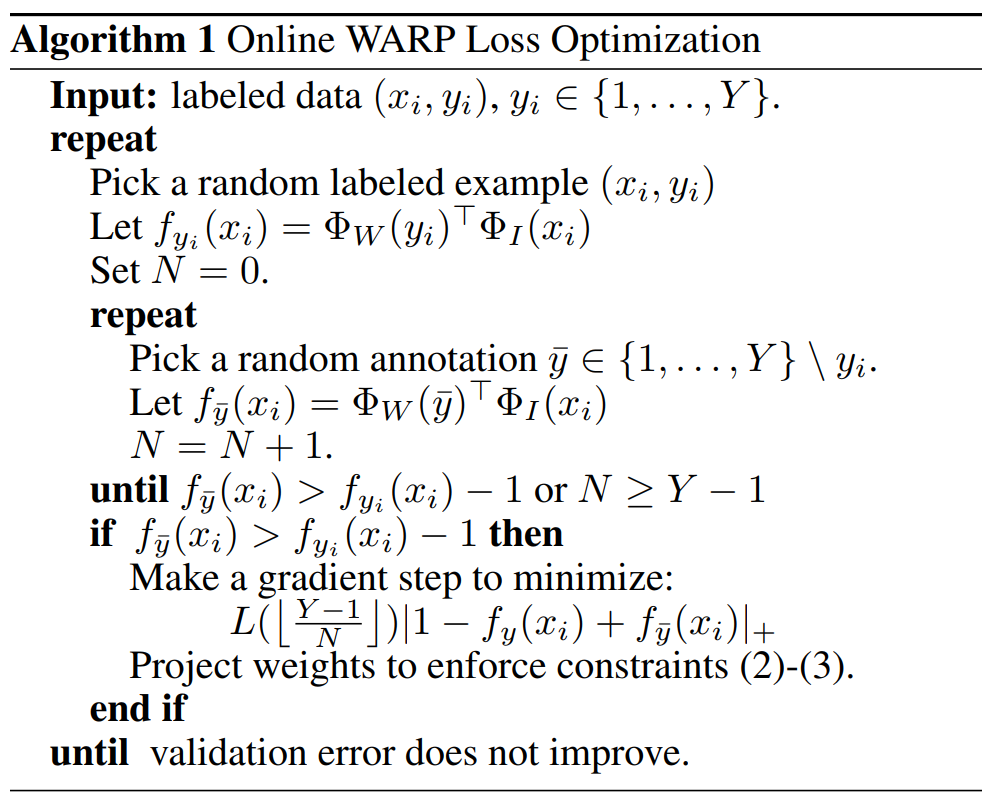
\includegraphics[max width=10cm,max height=10cm,keepaspectratio]{img_2_7}
	\caption[Online WARP Loss Optimization]{Online WARP Loss Optimization. Imagine preluată din \hyperlink{JasonWestonSamyBengioNicolasUsunier}{[8]}.}
\end{figure} 

\vspace{5mm}
\subsubsection*{k-OS WARP}
De completat ...

\section{Modelul LightFM}
Modelul LightFM este un model hibrid de matrix factorisation în care utilizatorii și articolele sunt reprezentate sub formă de combinații liniare de factorilor latenți a caracteristicilor. Modelul fiind hibrid, utilizează două strategii de învățare și anume învățarea coloborativă și filtrarea bazată pe conținut.

\vspace{5mm}
Cerințele de la care a fost dezvoltată structura modelului LightFM sunt \hyperlink{maciejlightfm}{[18]}:
\begin{enumerate}
	\item Modelul trebui să învețe reprezentările utilizatorilor și articolele din datele de interacțiune: această cerință este realizată prin utilizarea reprezentărilor latente. De exemplu, dacă două articole, fie $X$ și $Y$ sunt apreciate de aceași utilizatori, atunci reprezentările celor două articole, $X$ și $Y$, vor fi apropiate. Pe de altă parte, dacă articolele $X$ și $Y$ nu sunt apreciate de aceași utilizatori, atunci reprezentările celor două articole vor fi îndepărtate. Astfel, dacă reprezentările celor două articole $X$ și $Y$ sunt similare putem recomanda cu un grad ridicat de încredere articolul $Y$ unui utilizator dacă acel utilizator a interacționat cu articolul $X$;
	\item Modelul trebuie să poată face recomandări pentru articole și utilizatori noi: această cerință este indeplinită cu ajutorul prin reprezentarea articolelor și utilizatorilor sub formă de combinații liniare a caracteristicilor. Se aplică această abordare deoarece caracteristicile unui articol sau utilizator sunt cunoscute în momentul în care intră în sistem (de cele mai multe ori). De exemplu, Un film științifico-fantastic cu Leonardo DiCaprio poate fi reprezentat ca sumă a reprezentării genului științifico-fantastic și a reprezentării actorului Leonardo DiCaprio. Unu utilizator masculin din România poate fi reprezentat ca sumă a reprezentării utilizatorilor masculini și reprezentării țării România.
\end{enumerate}

\vspace{5mm}
Din punct de vedere formal modelul LightFM este definit după cum urmează în continuare \hyperlink{maciejlightfm}{[18]}.
Fie $U$ mulțimea de utilizatori, $I$ mulțimea de articole, $F^U$ mulțimea caracteristicilor utilizatorilor, $F^I$ mulțimea caracteristicilor articolelor. Fiecare utilizator interacționează cu un număr de elemente prin interacțiuni pozitive sau prin interacțiuni negative. Mulțimea tuturor interacțiunilor user - articol este definită ca $(u,i) \in U \times I$, unde în această reuniune sunt incluse atât interacțiunile pozitive cât și interacțiunile negative.

Utilizatorii și articolele sunt complet descrise de caracteristicile lor. Fiecare user $u$ este descris de un set de caracteristici $f_u \subset F^U$. Similar și pentru fiecare articol $i$, este descris de un set de caracteristici $f_i \subset F^I$. Caracteristicile sunt cunoscute dinainte și sunt reprezentate de metadatelor utilizatorilor sau articolelor.

Modelul este parametrizat d-dimensional pentru caracteristicile encodate ale utilizatorilor și articolelor și anume $e_f^U$ și $e_f^I$ pentru fiecare caracteristică $f$. Fiecărui feature i se mai adaugă un bias, $b_f^U$ pentru caracteristicile utilizatorilor și $b_f^I$ pentru caracteristicile articolelor.

Reprezentarea latentă a unui utilizator $u$ este dată de suma vectorilor latenți de caracteristici:
\begin{align}
	q_u = \sum_{j \in f_u} e_j^U
\end{align}
Similar și pentru articolul $i$:
\begin{align}
	p_i = \sum_{j \in f_i} e_j^I
\end{align}
Biasul pentru utilizatorul $u$ este dat de suma biasurilor caracteristicilor:
caracteristici:
\begin{align}
	b_u = \sum_{j \in f_u} b_j^U
\end{align}
Similar și pentru articolul $i$:
\begin{align}
	b_i = \sum_{j \in f_i} b_j^I
\end{align}

Predicția modelului pentru utilizatorul $u$ și articolul $i$ este dată de produsul dintre reprezentarea utilizatorului și reprezentarea articolului, ajustată cu biasurile pentru utilizator și articol:
\begin{align}
	\hat{r_{ui}} = f(q_u \cdot p_i + b_u + b_i)
\end{align}
unde $f$ poate fi reprezentat de multe tipuri de funcții, însă în acest model $f$ este setat ca fiind funcția sigmoid:
\begin{align}
	f(x) = \frac{1}{1 + exp(-x)}
\end{align}

Obiectivul de optimizare al modelului constă în maximizarea probabilității următoare:
\begin{align}
	L(e^U, e^I, b^U, b^I) = \prod_{(u,i) \in S^+} \hat{r}_{ui} \times \prod_{(u,i) \in S^-} (1 -\hat{r}_{ui})
\end{align}

\section{Rețele neurale convoluționale}

\subsection{Noțiuni generale}

Rețelele neurale convoluționale sunt rețelele formate din neuroni ce învață ponderi ($w$) și baiasuri ($b$). Scopul rețelei convoluționale este de a primi o imagine la input și de a scoate la output un scor pentru fiecare clasă ce corespunde imaginii. 

Spre exemplu, la input se dă o imagine cu un autovehicul, iar rețeaua convoluțională poate spune că în imagine este o mașină în proporție de 80\%, un camion în proporție de 10\%, un avion în proporție de 6\%, o barcă în proporție de 3\% sau un cal în proporție de 1\%.
\begin{figure}[!h]
	\centering
	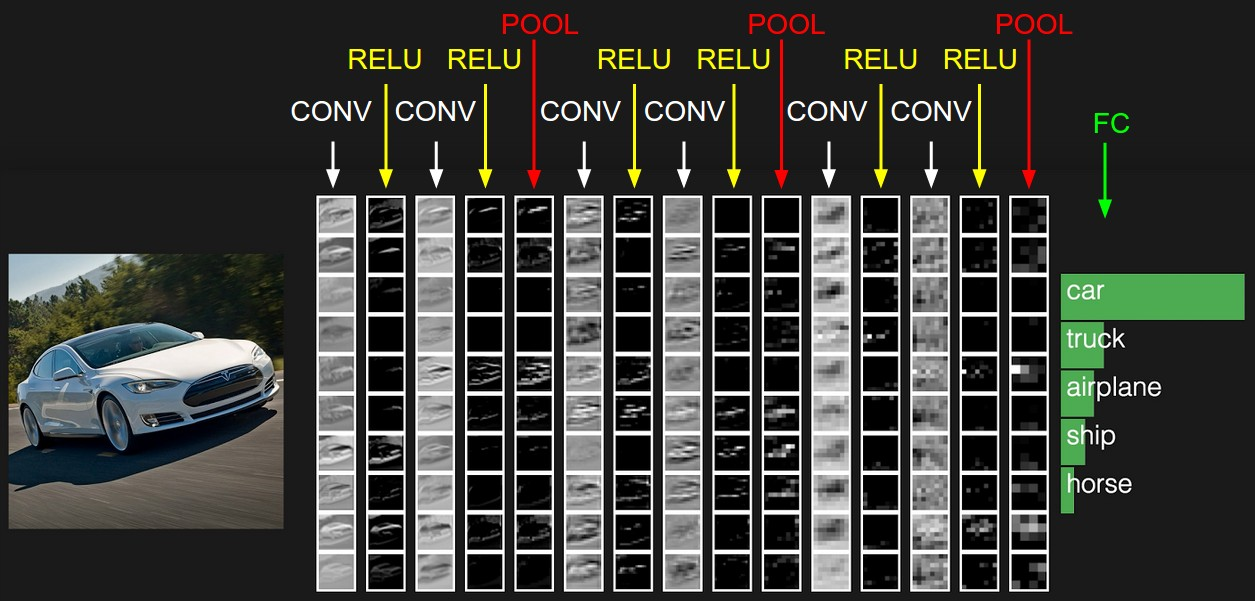
\includegraphics[max width=10cm,max height=10cm,keepaspectratio]{img_2_3}
	\caption[Exemplu rețea convoluțională]{Exemplu de rețea convoluțională care primește la input o imagine și produce la output o listă de clase ce pot descrie imaginea de input. Imagine preluată din \hyperlink{datameetsmedia}{[7]}.}
\end{figure} 

Rețelele convoluționale sunt compuse dintr-o secvență de straturi ce poate fi împărțită în trei tipuri principale \hyperlink{cs231n}{[7]}:
\begin{enumerate}
  \item Stratul convoluțional este stratul de bază într-o rețea. Parametrii acestui strat sunt reprezentați de filtre învățabile, unde fiecare filtru reprezintă o mică bucată din imaginea de input. De exemplu, un filtru pentru acest strat poate avea dimensiunea de $5 \times 5 \times 3$, dimensiune ce reprezintă faptul că se iau 5 pixeli pe lațime, 5 pixeli pe înălțime și o adâncime de 3 pixeli, unde adâncimea reprezintă canalele RGB. În continuare se glisează fiecare filtru peste input și se compune produsul dintre filtre și input la fiecare poziție. În urma acestei operații se produce un vector de activare 2-dimensional care reprezintă răspunsul filtrului la fiecare poziție. Altfel spun, rețeaua va învăța filtre care se activează atunci când sunt prezente anumite tipuri de caracteristici, precum culoarea sau orientarea (vezi figura 2.8).
\begin{figure}[!h]
	\centering
	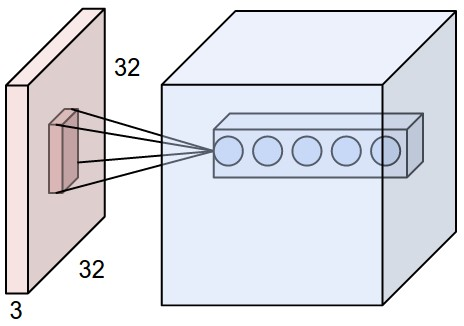
\includegraphics[max width=10cm,max height=10cm,keepaspectratio]{img_2_4}
	\caption[Exemplu de filtru aplicat peste input]{Exemplu de filtru aplicat peste input într-un strat convoluțional. Imagine preluată din \hyperlink{datameetsmedia}{[7]}.}
\end{figure}   
  
  \item Stratul de pooling reprezintă o practică des folosită între mai multe straturi convoluționale succesive. Această operație reduce numărul de parametrii (dimensiunea modelului), computațiile din rețea și controlează overfittingul. Se execută indepedent pe fiecare nivel al adâncimii unui input și pastrează valoarea maximă a acelei zone (de cele mai multe ori). Rezultatul este o zonă de caracteristicii mai mică dar care păstrează cea mai relevantă statistică (vezi figura 2.9).
\begin{figure}[!tbp]
  \begin{subfigure}[b]{0.4\textwidth}
    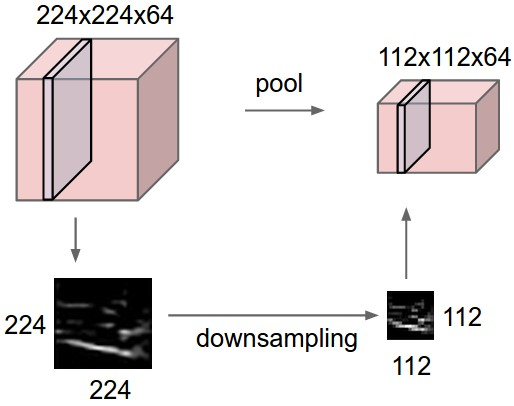
\includegraphics[width=\textwidth]{img_2_5}
    \caption{Reducerea dimensiunii.}
    \label{fig:f1}
  \end{subfigure}
  \hfill
  \begin{subfigure}[b]{0.4\textwidth}
    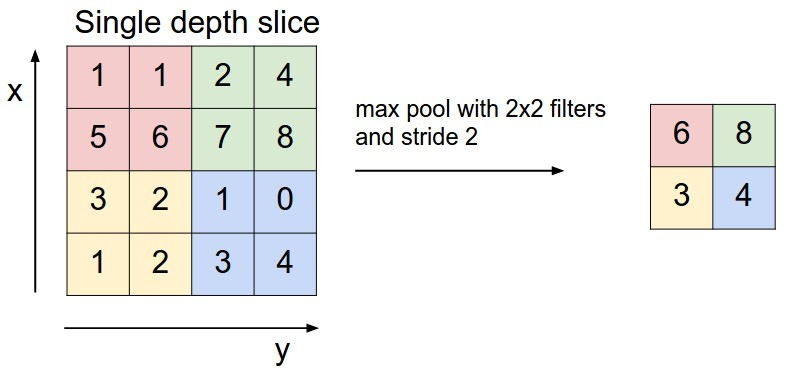
\includegraphics[width=\textwidth]{img_2_6}
    \caption{Filtrul de $2\times2$ aplicat ce păstrează valoarea maximă.}
    \label{fig:f2}
  \end{subfigure}
  \caption[Exemplu de pooling]{Exemplu de pooling. Imagine preluată din \hyperlink{datameetsmedia}{[7]}.}
\end{figure}
  
  \item Fully-Connected Layer este stratul în care caracteristicile sunt vectorizate pentru a putea fi folosite.
\end{enumerate}

\subsection{VGG}

VGG este o arhitectură clasică de rețea cu filtre convoluționale foarte mici, de dimensiune $3 \times 3$ și care poate avea un număr a straturilor de ponderi de 16 - 19. 

În ceea ce privește arhitectura (vezi figura 2.10), inputul în rețeaua convoluțională este de dimensiune fixă și anume $224 \times 224$ imagine RGB. Mai departe, imaginea este trecută printr-un set de straturi convoluționale unde sunt utilizate filtre de dimensiune mică, $3 \times 3$ - fiind cea mai mică dimensiune ce poate captura noțiunile de stânga/dreapta, sus/jos sau centru. Într-una dintre configurații se utilizează un filtru convoluțional de dimensiune $1 \times 1$. Pasul în straturile convoluționale este fixat la 1 pixel.

Poolingul este compus din cinci straturi de max-pooling care urmează după unele straturi convoluționale. Max-poolingul este calculat cu ferestre de $2\times2$ pixel și cu pas de 2 pixeli.

Odată trecută imaginea prin straturile convoluționale și cele de pooling ajunge în trei straturi fully-connected. Primele două straturi au câte 4096 de canale fiecare, iar al treilea are 1000 de canale. Canalele celui de-al treilea strat sunt asociate claselor, fiecare canal reprezintă o clasă.

Ultimul strat din rețea este un strat soft-max \hyperlink{SimonyanKarenZissermanAndrew}{[10]}.

\begin{figure}[!h]
	\centering
	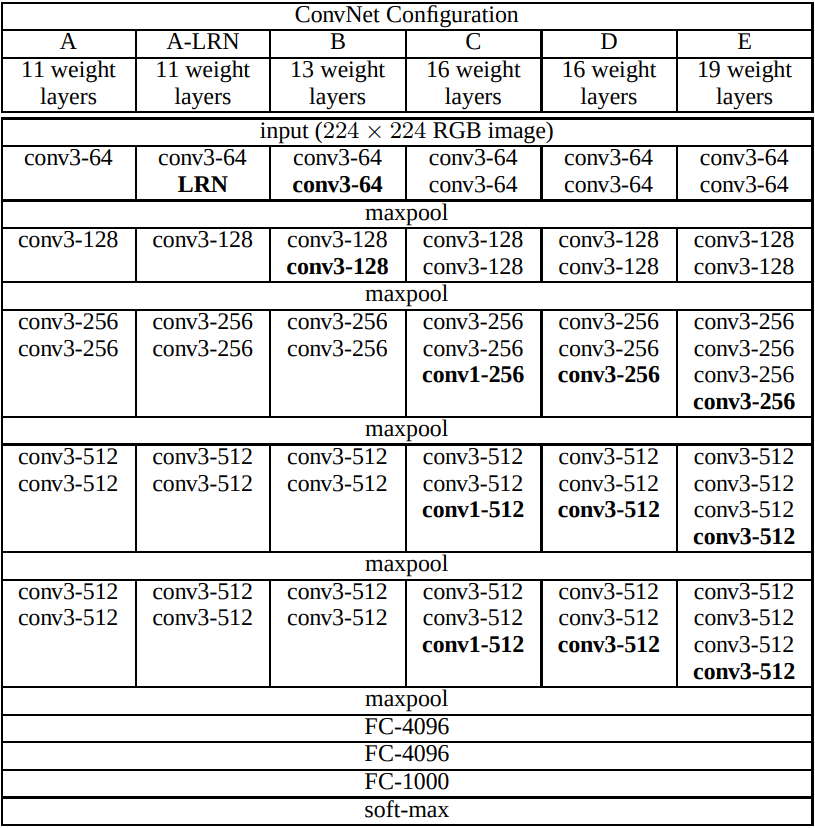
\includegraphics[max width=12cm,max height=12cm,keepaspectratio]{img_2_11}
	\caption[Configurații VGG]{Configurații ale rețelei VGG. Imagine preluată din \hyperlink{SimonyanKarenZissermanAndrew}{[10]}.}
\end{figure}   

\subsection{InceptionV3}
Prima arhitectura de Inception a apărut sub numele de GoogLeNet. O a doua versiune de Inception a fost definită prin introducerea de batch-uri normalizate. Iar mai apoi, versiunea a treia în care a fost adăugate idea de factorizare.

Factorizarea în filtre convoluționale mici (vezi figura 2.11) presupune înlocuirea stratului cu filtru de dimensiune $5 \times 5$ cu două straturi de dimensiune $3 \times 3$ astfel reducânduse dimensiunea de la $5 \times 5 = 25$ la $3 \times 3 + 3 \times 3 = 18$.
\begin{figure}[!h]
	\centering
	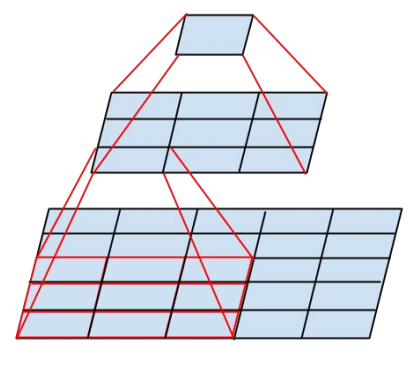
\includegraphics[max width=7cm,max height=7cm,keepaspectratio]{img_2_17}
	\caption[Factorizarea în filtre convoluționale mici]{Factorizarea în filtre convoluționale mici. Filtrul de dimensiune $5 \times 5$ înlocuit cu două de dimensiune $3 \times 3$. Imagine preluată din \hyperlink{guideinceptionv3}{[14]}.}
\end{figure}   

Factorizarea spațială în convoluții asimetrice (vezi figura 2.12) presupune înlocuirea stratului cu filtru de dimensiune $3 \times 3$ cu două straturi de dimensiune $3 \times 1$ și $1 \times 3$ astfel reducânduse dimensiunea de la $3 \times 3 = 9$ la $3 \times 1 + 1 \times 3 = 6$. 
\begin{figure}[!h]
	\centering
	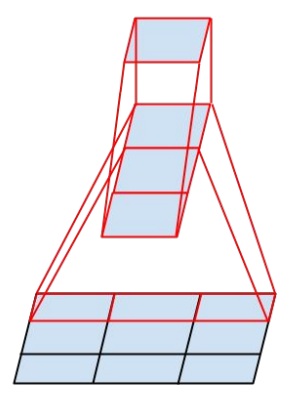
\includegraphics[max width=7cm,max height=7cm,keepaspectratio]{img_2_18}
	\caption[Factorizarea spațială în convoluții asimetrice]{Factorizarea în filtre convoluționale mici. Filtrul de dimensiune $3 \times 3$ înlocuit cu două de dimensiune $3 \times 1$ și $1 \times 3$.  Imagine preluată din \hyperlink{guideinceptionv3}{[14]}.}
\end{figure}

Clasificatorul auxiliar (vezi figura 2.13) este utilizat în InceptionV3 ca regulizator și este poziționat în partea superioară a utimelor $17 \times 17$ straturi. Batch-urile normalizate sunt de asemeanea folosite în clasificatorul auxiliar.
\begin{figure}[!h]
	\centering
	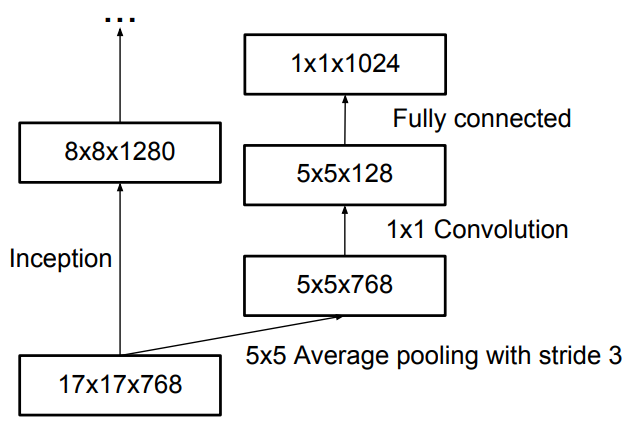
\includegraphics[max width=10cm,max height=10cm,keepaspectratio]{img_2_19}
	\caption[Clasificator auxiliar]{Clasificatorul auxiliar. Imagine preluată din \hyperlink{guideinceptionv3}{[14]}.}
\end{figure}

Reducerea eficientă a dimensiunii (vezi figura 2.14) se face prin utilizarea a două blocuri paralele, fie P și C. Primul dintre acestea, P, fiind un strat de activare de pooling (media sau maxim pooling). Ambele straturi au filtre cu pas 2 care sunt concatenate.
\begin{figure}[!h]
	\centering
	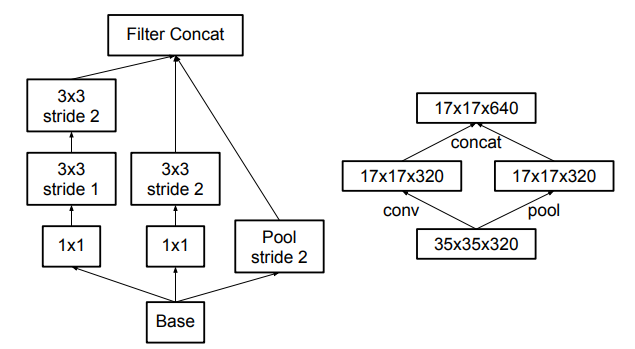
\includegraphics[max width=17cm,max height=12cm,keepaspectratio]{img_2_20}
	\caption[Reducerea eficientă a dimensiunii]{Modulul care reduce dimensiunea. Diagrama din dreapta reprezintă aceași soluție însă din perspectiva dimensiunii rețelei. Imagine preluată din \hyperlink{guideinceptionv3}{[14]}.}
\end{figure}   

Arhitectura completă este prezentată în figura 2.15.
\begin{figure}[!h]
	\centering
	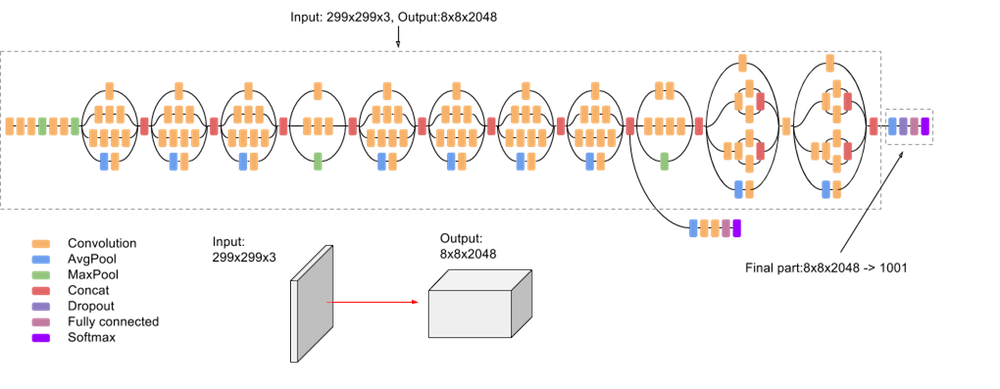
\includegraphics[max width=17cm,max height=12cm,keepaspectratio]{img_2_16}
	\caption[Arhitectura InceptionV3]{Arhitectura rețelei InceptionV3. Imagine preluată din \hyperlink{guideinceptionv3}{[14]}.}
\end{figure}   


\subsection{ResNet}
Fie $H(x)$ maparea de bază unde $x$ reprezintă inputul. Funcția reziduală poate fi aproximată cu $F(x) := H(x) - x$, maparea de bază fiind $F(x) + x$.

\begin{figure}[!h]
	\centering
	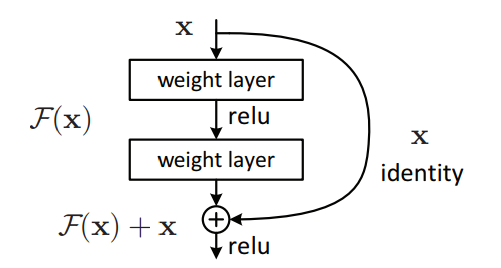
\includegraphics[max width=10cm,max height=10cm,keepaspectratio]{img_2_12}
	\caption[Învățarea reziduală]{Învățarea reziduală. Imagine preluată din \hyperlink{KaimingHeXiangyuZhangShaoqingRenJianSun}{[11]}.}
\end{figure}  

Învățarea reziduală se aplică la câtva grupuri de straturi. Putem defini un bloc de straturi ca fiind 
\begin{align}
	y = F(x,\{W_i\}) + x
\end{align}
unde $x$ și $y$ reprezintă inputul și outputul straturilor considerate. Funcția $F(x, \{W_i\})$ reprezintă maparea reziduală ce trebuie învățată.

Dimensiunea lui $x$ și $F$ din ecuația de mai sus trebuie să fie egale. Redefinim ecuația după cum urmează
\begin{align}
	y = F(x,\{W_i\}) + W_sx
\end{align}
unde $W_s$ este o proiecție liniară a scurtăturilor conexiunilor pentru ca dimensiunile să se potrivească.

ResNet (vezi figura 2.17) pleacă de la o rețea simplă. Rețeaua simplă fiind inspirată de rețeaua VGG. Straturile convoluționale au în general filtre de dimensiune $3 \times 3$ și se bazează de două reguli de design: - pentru outputuri cu același număr de caracteristici, straturile vor avea același număr de filtre; - dacă numărul de caracteristicii este injumătățit, numărul de filtre este dublat astfel încât să fie păstrată complexitatea de timp pe strat.

Poolingul se realizează dupa straturile convoluționale cu un pas de 2 pixeli. Rețeaua se termină cu un strat de pooling mediu și un strat fully-connected softmax cu 1000 de canale.

Bazată pe rețeaua descrisă mai sus, rețeaua reziduală presupune inserția unor scurtături. Scurtăturile identice (vezi formula 2.8) pot fi direct utilizate când inputul și outputul au aceași dimensiune. Când dimensiunea crește considerăm două opțiuni: - scurtătura calculează în continuare maparea identității. Această opțiune nu introduce parametrii noi; - proiecția scurtăturii din formula 2.9 este utilizată pentru a potrivi dimensiunile. În ambele situații când se folosesc scurtăturile pentru pentru a sări peste două straturi sunt calculate cu un pas de 2 pixeli.

\begin{figure}[!h]
	\centering
	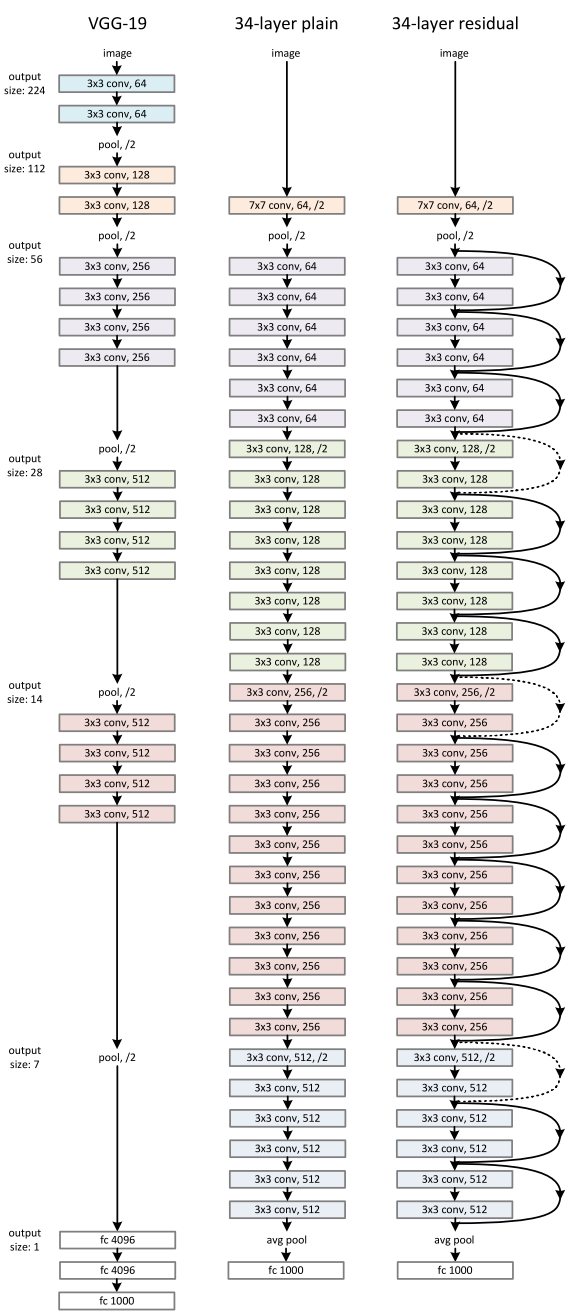
\includegraphics[max width=10cm,max height=20cm,keepaspectratio]{img_2_13}
	\caption[Rețeaua ResNet]{Prima rețea (stânga) este o rețea VGG19. A doua rețea (centru) este o rețea simplă cu 34 de straturi. A treia rețea (dreapta) este o rețea reziduală cu 34 de straturi. Imagine preluată din \hyperlink{KaimingHeXiangyuZhangShaoqingRenJianSun}{[11]}.}
\end{figure}  

\subsection{NASNet}
NASNet este o arhitectură de rețea bazată pe tehnica de căutare Neural Architecture Search (NAS, figura 2.18). NAS presupune un controler cu o rețea neurală recurentă care conține mai multe rețele copii cu arhitecturi diferite. Rețelele copii sunt antrenate să conveargă pentru a obține o anumită precizie pe un set de antrenare. Rezultatele sunt utilizate pentru a actualiza controlerul ceea ce înseamnă că acest controler va genera arhitecturi mai bune în timp.
\begin{figure}[!h]
	\centering
	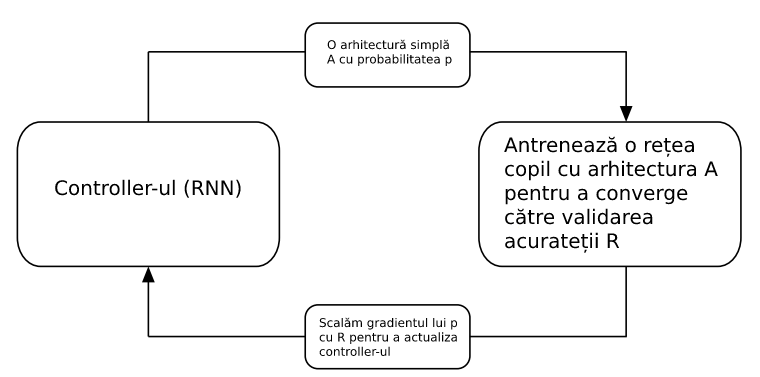
\includegraphics[max width=10cm,max height=20cm,keepaspectratio]{img_2_14}
	\caption[NAS]{Privire de ansamblu asupra unei Neural Architecture Search. Imagine preluată din \hyperlink{Zoph2018LearningTA}{[13]}.}
\end{figure}  

Plusul principal pe care îl aduce rețeaua NASnet este reprezentat de proiectarea unui nou spațiu de căutare astfel încât cea mai bună arhitectură pe setul de date CIFAR-10 poate scala către rezoluții ale imaginilor cât mai mari într-un interval definit. Astfel, acest spațiu poartă numele de \textit{NASNet search space}. În abordarea NASNet, arhitecturile rețelelor convoluționale sunt manual predeterminate, fiind compuse din celule convoluționale repetate de multe ori unde, fiecare celulă convoluțională are aceași arhitectură dar ponderi diferite.

Pentru a construi mai ușor arhitecturi scalabile pentru imagini de orice dimensiune este nevoie de două tipuri de celule convoluționale pentru a îndeplini două funcții principale: - celule convoluționale care returnează o hartă de caracteristici cu aceași dimensiune. Acest tip de celule se numește \textit{Celulă Normal}; - celule convoluționale care returnează o hartă de caracteristici cu înălțimea și lungimea harții divizată cu un factor doi. Acest tip de celule se numește \textit{Celulă de reducere} (vezi figura 2.19).
\begin{figure}[!h]
	\centering
	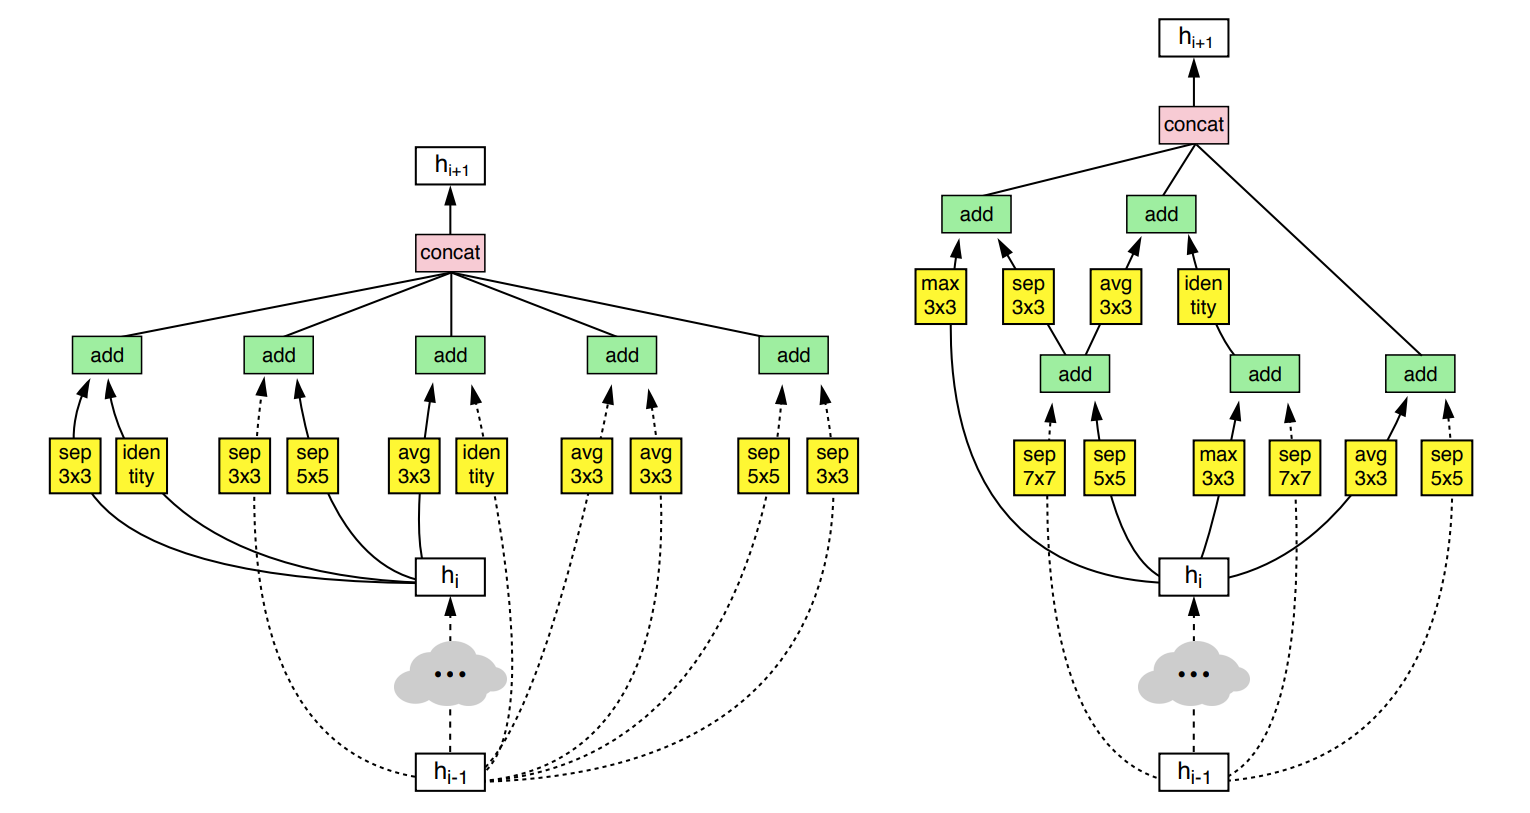
\includegraphics[max width=17cm,max height=17cm,keepaspectratio]{img_2_15}
	\caption[Celule normale și de reducere]{Celule normale (dreapta). Celule de reducere (stânga). Imagine preluată din \hyperlink{Zoph2018LearningTA}{[13]}.}
\end{figure}  

\section{Clustere}

\subsection{Noțiuni generale}

Clusterizarea este un proces de grupare a unor articole în sensul în care articolele din același cluster sunt foarte similare între ele din punct de vedere al caracteristicilor. Această metodă este des utilizată în data mining, analiza datelor, machine learning, recunoașterea tiparelor sau regăsirea informației. Există mai multe tipuri de algoritmi de clusterizare, însă, ideea de bază este aceași: clusterele sunt grupuri cu distanțe foarte mici între membrii grupului (fie distanța euclidiană, de exemplu).
\begin{figure}[!h]
	\centering
	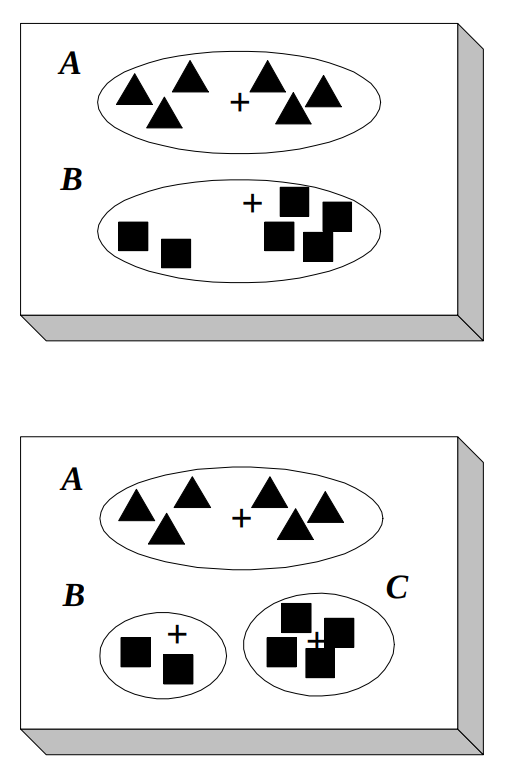
\includegraphics[max width=10cm,max height=10cm,keepaspectratio]{img_2_21}
	\caption[Exemplu clustere]{Exemplu de două clustere (sus). Exemplu de trei clustere (jos). Imagine preluată din \hyperlink{dataclusteringtechniques}{[15]}.}
\end{figure}  

Procesul de clustering poate fi împărțit în etape după cum urmează \hyperlink{dataclusteringtechniques}{[15]}:
\begin{enumerate}
	\item Colectarea datelor: alegerea articolelor pentru care se va aplica clusterizarea;
	\item Screening-ul inițial: presupune extragerea caracteristicilor relevante pentru fiecare articol din dataset;
	\item Reprezentarea: presupune pregătirea datelor pentru a putea fi folosite de către algoritmul de clusterizare, tot aici alegânduse și măsura de similaritate;
	\item Tendința de grupare: se verifică dacă datele au o tendință naturală de grupare; poate fi sărită pentru baze de date mari;
	\item Strategia de clusterizare: se alege algoritmul de clusterizare și parametrii inițiali;
	\item Validarea: se evaluează manual/vizual sau prin alte metode definite rezultatele obținute în urma clusterizări;
	\item Interpretarea: în această se compară rezultatele pe mai multe clustere, combinații de clustere și se trag concluziile.
\end{enumerate}

\subsection{K-nearest neighbors}
KNN reprezintă un model de clasificare simplu și eficient în multe cazuri. Pentru ca un articol $t$ să fie clasificat sunt căutați cei mai propiați $k$ vecini formând regiunea lui $t$. Cei mai apropiați veci sunt căutați cu o măsură de similaritate, de obicei distanța euclidiană sau similaritatea cosinus. Votul majoritar din acea regiune este folosit pentru a decide clasificarea lui $t$. $k$-ul este valoarea de care depinde destul de mult rata de succes a calsificării, cea mai simplă metodă de a alege un $k$ optim fiind reprezentată de rularea algoritmului pentru mai multe valori ale lui și observarea evoluției rezultelor.

\vspace{5mm}
Fie $D$ o colecție de $n$ clase cunoscute $\{d_1, d_2,..., d_n\}$. $Sim(d_i)$ - similaritatea celui mai indepărtat punct din regiunea locală, $N(d_i)$ - numărul de puncte din interiorul unei regiuni locale. Algoritmul de construcție al modelului este definit după cum urmează \hyperlink{gongdeguo}{[16]}:
\begin{enumerate}
	\item selectăm o măsură de similaritate și creem o matrice de similaritate peste baza de date de antrenare;
	\item setăm toate datele cu eticheta neclasificate;
	\item pentru fiecare intrare cu eticheta de neclasificat căutăm cea mai mare regiune locală care acoperă cel mai mare număr de vecini cu aceași categorie.
	\item căutam intrarea $d_i$ cu cea mai mare regiune $N_i$ printre toate regiunile locale și creem o reprezentare $<Cls(d_i), Sim(d_i), Num(d_i), Rep(d_i)>$ în modelul $M$ pentru a reprezenta toate intrările acoperite de regiunea $N_i$ și setăm etichete pentru toate aceste intrări;
	\item repetăm pași 3 și 4 până când toate intrările din baza de date de antrenare au fost clasificate;
	\item modelul $M$ este format din toate reprezentările setate în procesul de învățatare descris mai sus.
\end{enumerate}

Algoritmul de clasificare este definit după cum urmează:
\begin{enumerate}
	\item pentru ca o nouă intrare $d_t$ să fie clasificată, calculăm similaritatea ei cu toate celelalte reprezentări din model;
	\item dacă $d_t$ este acoperit doar de o reprezentare $<Cls(d_j), Sim(d_j), Num(d_j), Rep(d_j)>$ în sensul că distanța de la $d_t$ la $d_j$ este mai mică decât $Sim(d_j)$, $d_t$ este astfel clasificat ca făcând parte din clasa lui $d_j$;
	\item dacă $d_t$ este acoperit de două sau mai multe clase, clasificăm $d_t$ ca făcând parte din reprezentarea cu cea mai mare valoare a $Num(d_j)$, adică regiunea care acoperă cel mai mare număr de intrări din baza de date de antrenare;
	\item dacă nu există nicio reprezentare în modelul M care să acopere $d_t$, clasificăm $d_t$ cu o clasă nouă.
\end{enumerate}

Un exemplu vizual de execuție a algoritmului de kNN, parcurs pas cu pas, este prezentat în figura 2.21. Exemplu conține 36 de intrări din 2 clase marcate prin pătrat și cerc. Datele de test sunt reprezentate prin tringhiuri.
\begin{figure}[!tbp]
  \begin{subfigure}[b]{0.4\textwidth}
    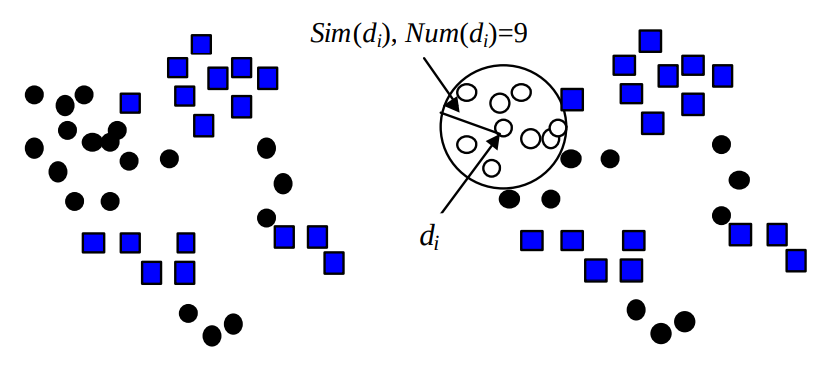
\includegraphics[width=\textwidth]{img_2_22}
    \caption{Distribuția inițială a datelor (stânga) și prima reprezentare obținută (dreapta)}
    \label{fig:f1}
  \end{subfigure}
  \hfill
  \begin{subfigure}[b]{0.4\textwidth}
    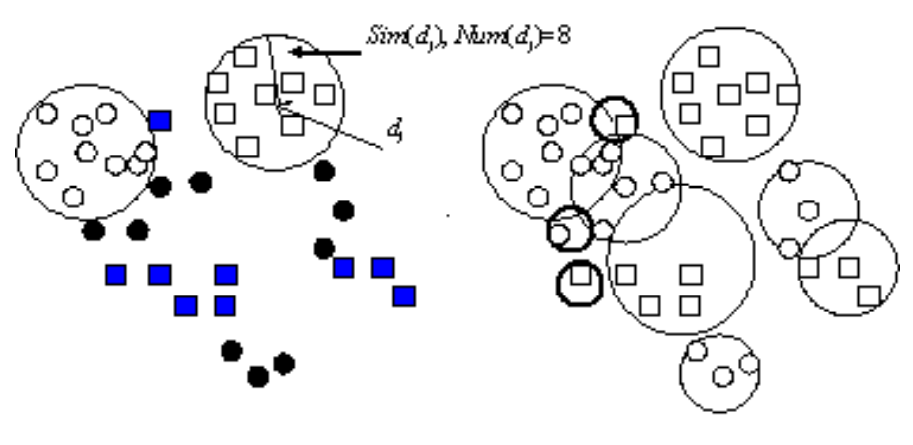
\includegraphics[width=\textwidth]{img_2_23}
    \caption{A doua reprezentare obținută (stânga) și modelul înainte de triere (dreapta)}
    \label{fig:f2}
  \end{subfigure}
  \hfill
  \begin{subfigure}[b]{0.4\textwidth}
    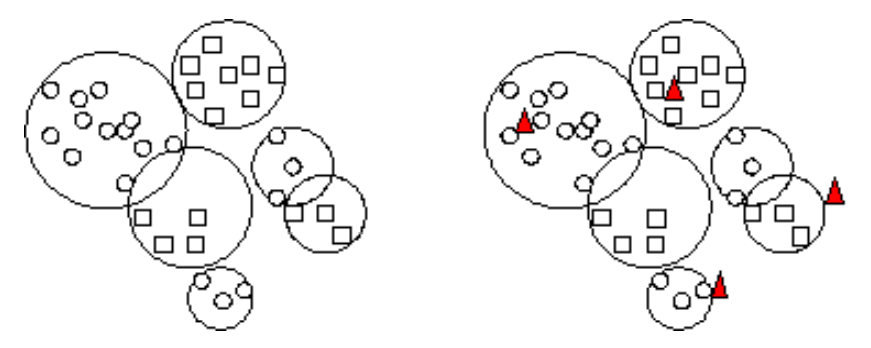
\includegraphics[width=\textwidth]{img_2_24}
    \caption{Modelul după triere (stânga) și distribuția datelor de test (dreapta)}
    \label{fig:f3}
  \end{subfigure}
  \caption[Exemplu 1 de clasificare cu kNN]{Exemplu 1 de clasificare cu kNN. Imagine preluată din \hyperlink{gongdeguo}{[16]}.}
\end{figure}  

Un al doilea exemplu de clasificare este prezentat în figura 2.22:
\begin{figure}[!tbp]
  \begin{subfigure}[b]{0.4\textwidth}
    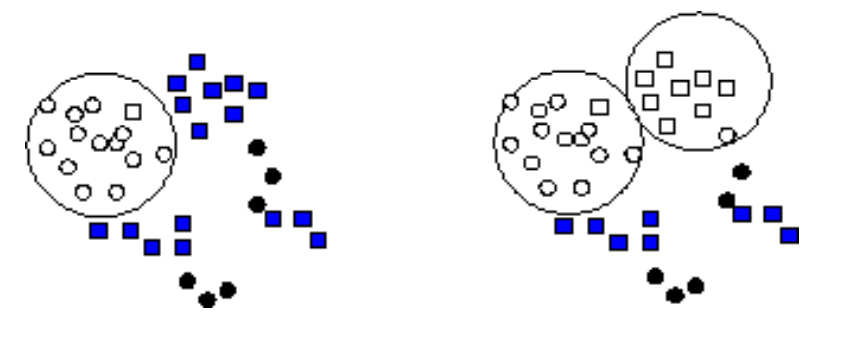
\includegraphics[width=\textwidth]{img_2_25}
    \caption{Prima reprezentare obținută (stânga) și a doua reprezentare obținută(dreapta)}
    \label{fig:f1}
  \end{subfigure}
  \hfill
  \begin{subfigure}[b]{0.4\textwidth}
    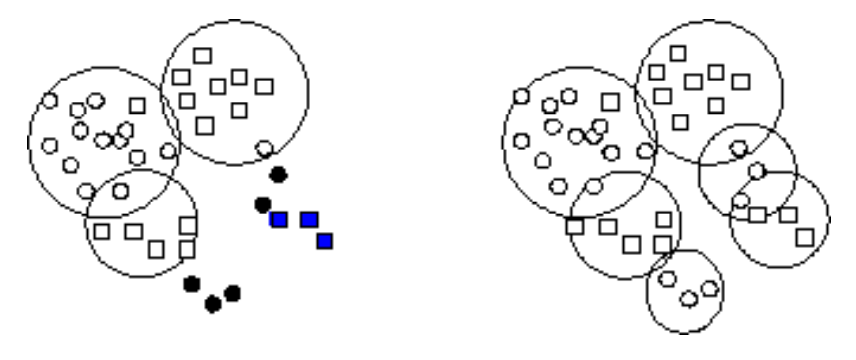
\includegraphics[width=\textwidth]{img_2_26}
    \caption{A treia reprezentare obținută (stânga) și modelul final (dreapta)}
    \label{fig:f2}
  \end{subfigure}
  \caption[Exemplu 2 de clasificare cu kNN]{Exemplu 2 de clasificare cu kNN. Imagine preluată din \hyperlink{gongdeguo}{[16]}.}
\end{figure}

\subsection{Metrici de evaluare a clusterelor}

\subsubsection{Coeficientul silhouette}

Coeficient (vezi formula 2.10) este folosit pentru a evalua clusterele în învățarea nesupervizată. Este calculat utilizând distanța euclidiană medie intra-clustere ($a$) și distanța medie către cel mai apropiat cluster ($b$) pentru fiecare intrare, adică distanța dintre o intrare și cel mai apropiat cluster din care nu face parte. Numărul de etichete trebuie să respecte constrangerea $2 \leq nr_{etichete} \leq nr_{etichete} - 1$. Valorile returnate de acest coeficient sunt cuprinse în intervalul $[-1, 1]$. Valorile apropiate de 0 indică clustere care se suprapun, valorile negative în general indică că există intrări asignate în clusterul greșit, iar valorile apropiate de 1 indică o separație bună intre clustere \hyperlink{silhouette}{[17]}.
\begin{align}
	\frac{b-a}{max(a,b)}
\end{align}
